\documentclass[12pt,a4paper]{article}
\usepackage[MeX]{polski}
\usepackage[utf8]{inputenc}
\usepackage{listings}
\usepackage{graphicx}
\usepackage{fancyvrb}
\usepackage{tabularx}
\usepackage{geometry}
\usepackage{multirow}
\geometry{
 a4paper,
 total={170mm,257mm},
 left=20mm,
 top=20mm,
}
\author{Yurii~Vyzhha}
\title{Metody Obliczeniowe w Nauce i Technice \\ Laboratorium 1 \\
  Arytmetyka Komputerowa \\ Sprawozdanie}
\begin{document}
  \maketitle
  \paragraph{Zadanie 1 Sumowanie liczb pojedynczej precyzji}\mbox{}\vspace{3mm}\\
  \emph{Zwykły algorytm sumowania}
  \begin{Verbatim}[fontsize=\footnotesize]
  float[] ar = new float[10000000];
  float v = 0.53125f;
  for (int i = 0; i < ar.length; i++) {
      ar[i] = v;
  }
  float sum = 0.0f;
  for (int i = 0; i < ar.length; i++) {
      sum += ar[i];
  }
  \end{Verbatim}
  Bezwzględny błąd: $ \sim 5.3 \%$. \\
  Względny błąd: $ 281659.5$. \\
  Wielkość błędu sumowania jest związana z reprezentacją liczb
  zmiennoprzecinkowych oraz z implementacją sumowania dwóch l.z.
  Dla obliczenia sumy dwóch l.z. mantysę mniejszej z liczb musimy doprowadzić
  do postaci większej z liczb co wiąże się z utratą mniej znaczących cyfr
  cechy. \\
  Poniżej przedstawiamy wykres który pokazuje zależność pomiędzy błędem
  bezwzględnym a ilością iteracji wykonanych przez program.\\
  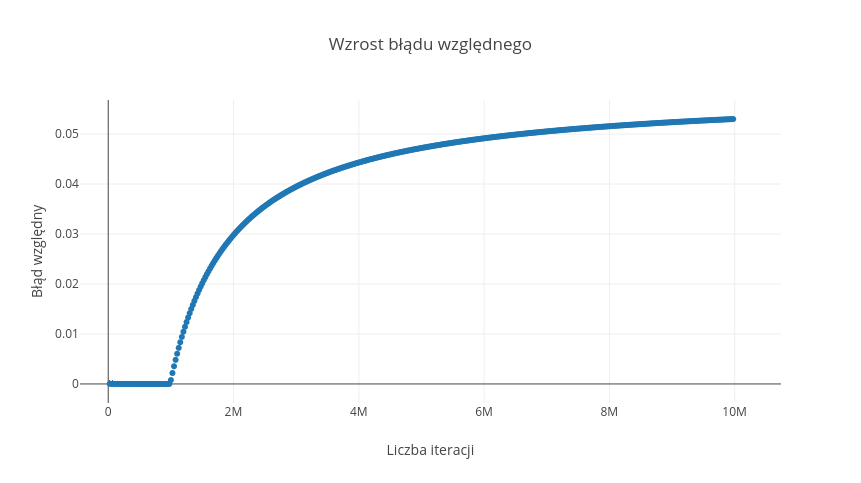
\includegraphics[width=0.9\textwidth]{img/Plot1} \\
  Jak widzimy na wykresie, przy pierwszych $10^6$ iteracji nie mamy błędu.
  To jest związane z tym, że wielkość cechy jest wystarczają duża, a różnica
  między liczbami, które dodajemy, jest wystarczająco mała. Później błąd
  bezwględny się pojawia, ale rośnie co raz z mniejszą prędkością. To jest
  spowodowane tym, że z każdym dodawaniem mylimy się na stałą liczbę, a suma
  rośnie, więc udział błędu w sumie jest co raz mniejszy.\vspace{3mm}\\
  \emph{Rekurencyjny algorytm dodawania}
  \begin{Verbatim}[fontsize=\footnotesize]
  public static float recSum(float[] ar, int a, int b) {
      if (a == b) return ar[a];
      if (b - a == 1) {
          return ar[a] + ar[b];
      }
      return recSum(ar, a, (b + a)/2) + recSum(ar, (b + a)/2 + 1, b);
  }
  \end{Verbatim}
  Bezwzględny błąd: $ 0.0 \% $. \newline
  Względny błąd: $ 0.0 $. \newline
  Korzystając z rekurencyjnego algorytmu, nie dostaliśmy błędu. Ten algorytm
  jest zaimplementowany tak, że dodaje liczby wylącznie o tej samej wielkości,
  więc przesunięcie cechy i, co za tym idzie, utrata precyzji nie występują.
  \newline
  Czas działania obu algorytmów jest mniej więcej taki sam dla różnych danych
  wejściowych.
  \paragraph{Zadanie 2 Algorytm Kahana}\mbox{}\vspace{3mm}\\
  \emph{Implementacja algorytmu Kahana w języku Java}
  \begin{Verbatim}[fontsize=\footnotesize]
      float sum = 0.0f;
      float err = 0.0f;
      for (int i = 0; i < ar.length; i++) {
          float y = ar[i] - err;
          float temp = sum + y;
          err = (temp - sum) - y;
          sum = temp;
      }
  \end{Verbatim}
  Algorytm Kahana działa w następujący sposób. Każdego razu jak dodajemy
  nową liczbę do ogólnej sumy ($sum + y$), obliczamy korektę ($err$),
  który stosujemy w następnej iteracji. Najpierw odejmujemy korektę $err$,
  którą obliczyliśmy w poprzedniej iteracji pętli i otrzymujemy poprawiony
  składnik $y$. Później dodajemy ten składnik do sumy $sum$. Najmniej znaczące
  bity $y$ straciliśmy przy sumowaniu. Potem obliczamy najbardziej znaczące
  bity $y$ za pomocą $temp - sum$. Kiedy odejmniemy $y$ od otrzymanej różnicy,
  odzyskamy najmniej znaczące bity. Te właśnie bity straciliśmy przy obliczaniu
  $sum + y$. One będą korektą w następnej iteracji. \newline
  Czas działania algorytmów Kahana oraz rekurencyjnego jest mniej więcej taki
  sam dla różnych danych wejściowych.
  \paragraph{Zadanie 3 Sumy częściowe}\mbox{}\vspace{3mm}\\
  Tablice nalerzy czytać w następujący sposób: najpierw podany jest wynik,
  otrzymany przy sumowaniu wprzód, a niżej w tej samej komórce wynik, otrzymany
  przy sumowaniu wstecz.
  \emph{Funkcje policzone z pojedynczą precyzją:} \vspace{3mm}\\
  Funkcja dzeta Riemanna: \vspace{3mm}\newline
  \begin{tabularx}{\textwidth}{ |l|l|X|X|X|X|X| }
      \hline
      & & \multicolumn{5}{ c| }{n} \\ \hline
      & & 50 & 100 & 200 & 500 & 1000 \\ \hline
      \multirow{5}{*}{s} & 2 & 1.6251329 1.6251328 & 1.634984 1.6349839 & 1.6399467 1.6399465 & 1.642936 1.642936 & 1.6439348 1.6439345 \\ \cline{2-7}
      & 3.6667 & 1.1093994 1.1093998 & 1.1094086 1.1094089 & 1.1094086 1.1094103 & 1.1094086 1.1094105 & 1.1094086 1.1094105 \\ \cline{2-7}
      & 5 & 1.0369275 1.0369277 & 1.0369275 1.0369277 & 1.0369275 1.0369277 & 1.0369275 1.0369277 & 1.0369275 1.0369277 \\ \cline{2-7}
      & 7.2 & 1.0072277 1.0072277 & 1.0072277 1.0072277 & 1.0072277 1.0072277 & 1.0072277 1.0072277 & 1.0072277 1.0072277 \\ \cline{2-7}
      & 10 & 1.0009946 1.0009946 & 1.0009946 1.0009946 & 1.0009946 1.0009946 & 1.0009946 1.0009946 & 1.0009946 1.0009946 \\
      \hline
  \end{tabularx} \vspace{3mm}\newline
  Funkcja eta Dirichleta: \vspace{3mm}\newline
  \begin{tabularx}{\textwidth}{ |l|l|X|X|X|X|X| }
      \hline
      & & \multicolumn{5}{ c| }{n} \\ \hline
      & & 50 & 100 & 200 & 500 & 1000 \\ \hline
      \multirow{5}{*}{s} & 2 & 0.822271 0.82227105 & 0.8224175 0.8224175 & 0.8224547 0.8224546 & 0.82246536 0.82246506 & 0.82246685 0.8224665 \\ \cline{2-7}
      & 3.6667 & 0.93469304 0.93469304 & 0.9346932 0.93469334 & 0.9346932 0.93469334 & 0.9346932 0.93469334 & 0.9346932 0.93469334 \\ \cline{2-7}
      & 5 & 0.9721198 0.97211975 & 0.9721198 0.97211975 & 0.9721198 0.97211975 & 0.9721198 0.97211975 & 0.9721198 0.97211975 \\ \cline{2-7}
      & 7.2 & 0.99352705 0.993527 & 0.99352705 0.993527 & 0.99352705 0.993527 & 0.99352705 0.993527 & 0.99352705 0.993527 \\ \cline{2-7}
      & 10 & 0.99903953 0.99903953 & 0.99903953 0.99903953 & 0.99903953 0.99903953 & 0.99903953 0.99903953 & 0.99903953 0.99903953 \\
      \hline
  \end{tabularx} \vspace{3mm}\newline
  \emph{Funkcje policzone z podwójną precyzją:} \vspace{3mm}\\
  Funkcja dzeta Riemanna: \vspace{3mm}\newline
  \begin{tabularx}{\textwidth}{ |l|l|X|X|X| }
      \hline
      & & \multicolumn{3}{ c| }{n} \\ \hline
      & & 50 & 100 & 200 \\ \hline
      \multirow{5}{*}{s} & 2 & 1.625132733621529 1.6251327336215293 & 1.6349839001848923 1.634983900184893 & 1.6399465460149971 1.6399465460149973 \\ \cline{2-5}
      & 3.6667 & 1.1093997551541945 1.1093997551541943 & 1.1094087973421474 1.1094087973421476 & 1.1094102423332313 1.109410242333231 \\ \cline{2-5}
      & 5 & 1.036927716716712 1.0369277167167108 & 1.0369277526929555 1.0369277526929532 & 1.0369277549886775 1.036927754988676 \\ \cline{2-5}
      & 7.2 & 1.0072276664762816 1.0072276664762823 & 1.007227666480654 1.007227666480655 & 1.0072276664807145 1.0072276664807163 \\ \cline{2-5}
      & 10 & 1.0009945751278182 1.000994575127818 & 1.0009945751278182 1.000994575127818 & 1.0009945751278182 1.000994575127818 \\
      \hline
  \end{tabularx} \vspace{3mm}\newline
  \begin{tabularx}{\textwidth}{ |l|l|X|X| }
      \hline
      & & \multicolumn{2}{ c| }{n} \\ \hline
      & & 500 & 1000 \\ \hline
      \multirow{5}{*}{s} & 2 & 1.642936065514894 1.6429360655148941 & 1.6439345666815615 1.6439345666815597 \\ \cline{2-4}
      & 3.6667 & 1.1094104908440712 1.1094104908440725 & 1.1094105108423578 1.1094105108423593 \\ \cline{2-4}
      & 5 & 1.0369277551393863 1.0369277551393858 & 1.0369277551431222 1.0369277551431204 \\ \cline{2-4}
      & 7.2 & 1.0072276664807145 1.0072276664807172 & 1.0072276664807145 1.0072276664807172 \\ \cline{2-4}
      & 10 & 1.0009945751278182 1.000994575127818 & 1.0009945751278182 1.000994575127818 \\
      \hline
  \end{tabularx} \vspace{3mm}\newline
  Funkcja eta Dirichleta: \vspace{3mm}\newline
  \begin{tabularx}{\textwidth}{ |l|l|X|X|X| }
      \hline
      & & \multicolumn{3}{ c| }{n} \\ \hline
      & & 50 & 100 & 200 \\ \hline
      \multirow{5}{*}{s} & 2 & 0.8222710318260295 0.8222710318260289 & 0.8224175333741286 0.8224175333741282 & 0.822454595922551 0.8224545959225509 \\ \cline{2-5}
      & 3.6667 & 0.9346930600307106 0.934693060030711 & 0.9346933211400662 0.934693321140067 & 0.9346933421086845 0.9346933421086852 \\ \cline{2-5}
      & 5 & 0.9721197689267979 0.9721197689267976 & 0.9721197703981592 0.9721197703981589 & 0.972119770445367 0.9721197704453663 \\ \cline{2-5}
      & 7.2 & 0.9935270006613486 0.9935270006613481 & 0.9935270006616185 0.9935270006616179 & 0.9935270006616201 0.9935270006616198 \\ \cline{2-5}
      & 10 & 0.9990395075982718 0.9990395075982715 & 0.9990395075982718 0.9990395075982715 & 0.9990395075982718 0.9990395075982715 \\
      \hline
  \end{tabularx} \vspace{3mm}\newline
  \begin{tabularx}{\textwidth}{ |l|l|X|X| }
      \hline
      & & \multicolumn{2}{ c| }{n} \\ \hline
      & & 500 & 1000 \\ \hline
      \multirow{5}{*}{s} & 2 & 0.8224650374240963 0.8224650374240972 & 0.8224665339241114 0.8224665339241127 \\ \cline{2-4}
      & 3.6667 & 0.9346933438558745 0.934693343855875 & 0.9346933439141353 0.9346933439141354 \\ \cline{2-4}
      & 5 & 0.9721197704468947 0.9721197704468933 & 0.9721197704469091 0.9721197704469088 \\ \cline{2-4}
      & 7.2 & 0.9935270006616201 0.9935270006616198 & 0.9935270006616201 0.9935270006616198 \\ \cline{2-4}
      & 10 & 0.9990395075982718 0.9990395075982715 & 0.9990395075982718 0.9990395075982715 \\
      \hline
  \end{tabularx} \vspace{3mm}\newline
\end{document}
